\chapter{The GLLAMM for dichotomous outcomes} \label{chap:framework}

The Generalized Linear Latent and Mixed Model (GLLAMM) is a framework that unifies a wide range of latent variable models. Developed by Rabe-Hesketh and colleagues \cite{Rabe_et_al_2004a, Rabe_et_al_2004b, Rabe_et_al_2004c, Skrondal_et_al_2004a, Rabe_et_al_2012}, the method was motivated by the need of a Multilevel Structural Equation Model (MSEM) that accommodated for unbalanced data, noncontinuous responses and cross-level effects among latent variables. The authors focused its development mainly from the frequentist perspective, however, they offered a general guidance on implementing the model under the bayesian framework (see \citet{Skrondal_et_al_2004a}).

%%%%%%%%%%%%%%%%%%%%%%%%%%%%%%%%%%%%%%%%%%%%%%%%%%%%%%%%%%%%%%%%%%%%%%%
%%%%%%%%%%%%%%%%%%%%%%%%%%%%%%%%%%%%%%%%%%%%%%%%%%%%%%%%%%%%%%%%%%%%%%%

\section{Model motivation} \label{sect:motivation}

Consider a large standardized assessment composed of three sub-test designed to evaluate the reading comprehension, mathematical reasoning, and pedagogical knowledge of teachers; where each sub-test has several dichotomously scored items. 

Focusing on the first sub-test, the items were designed to measure only one of the three hierarchically nested sub-dimensions of reading comprehension: literal, inferential, and reflective abilities. Furthermore, it is assumed the three sub-dimensions are all that is needed to measure the reading comprehension ability, effectively making this scale, the highest level latent variable in the model, similar to a hierarchical Confirmatory Factor Analysis (CFA). Finally, the items were bundled in groups of five to a common text or passage, i.e. testlets, that provided the stimulus over which the individual is assessed. Figure \ref{fig:design} shows the path diagram of the hypothesized dimensional structure, for the hierarchical cross-classified IRT model corresponding with the instrument. The figure represents the responses of one person on $12$ items.
%
\begin{figure}[h]
	\centering
	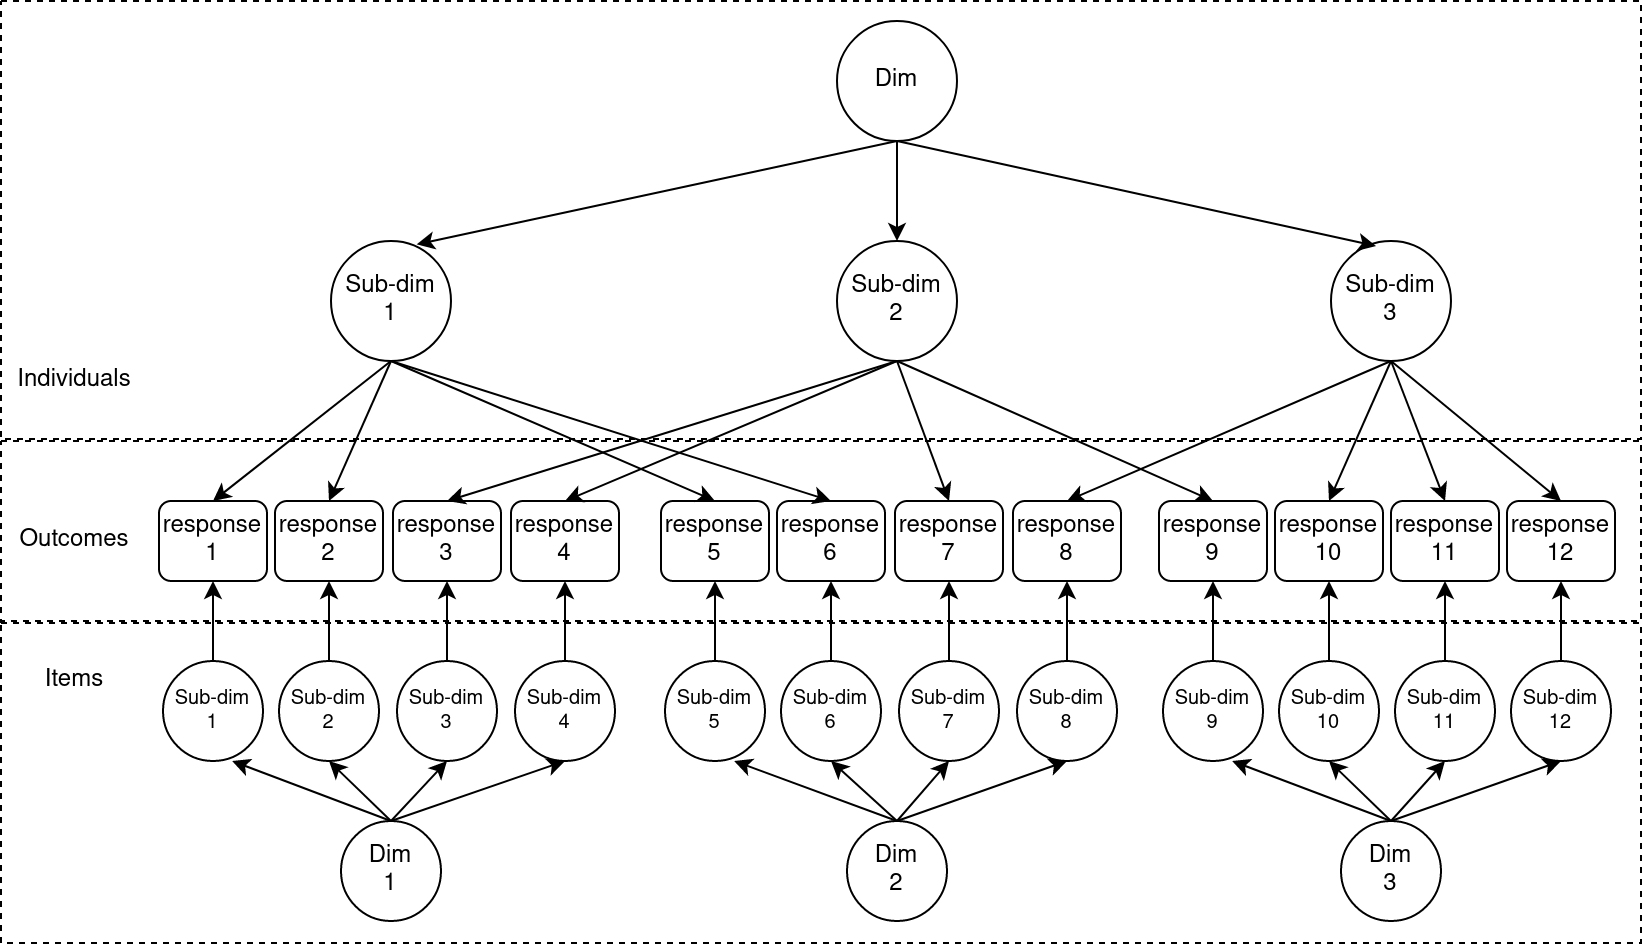
\includegraphics[width=0.9\textwidth]{instrument_design}
	\caption[Path diagram of the dimensional structure for a hierarchical cross-classified IRT model.]%
	{Path diagram of the dimensional structure for a hierarchical cross-classified IRT model. Squares represent dichotomous manifest variables, and circles represent latent variables. The figure is based on a reduced set of items, while the errors and scales of the latent variables are not represented. Different sub-dimensions at the individuals block represent the literal, inferential and reflective abilities, while at the items blocks represent the items' difficulties. The dimensions at the individuals block represent the reading comprehension ability, while at the items block represent the multiple testlets.}
	\label{fig:design}
\end{figure}

With the purpose of providing an easier motivation of the model, we will not consider yet the cluster effects; however, later in the presentation we will show how easy it is to introduce them in the model. Just for future reference, under this example, one expects to observe clustering effects, because individuals from different regions did not have the same educational opportunities, effectively causing differences among them at a regional level.

%%%%%%%%%%%%%%%%%%%%%%%%%%%%%%%%%%%%%%%%%%%%%%%%%%%%%%%%%%%%%%%%%%%%%%%
%%%%%%%%%%%%%%%%%%%%%%%%%%%%%%%%%%%%%%%%%%%%%%%%%%%%%%%%%%%%%%%%%%%%%%%

\section{Model definition} \label{sect:definition}

Following \citet{Rabe_et_al_2004a, Rabe_et_al_2004b}, we continue defining the GLLAMM in two parts: (i) the response model, and (ii) the latent structure.

In case the reader is interested in outcomes different than the dichotomous case, refer to Appendix \ref{appA1:links}.

%%%%%%%%%%%%%%%%%%%%%%%%%%%%%%%%%%%%%%%%%%%%%%%%%%%%%%%%%%%%%%%%%%%%%%%

\subsection{Response model} \label{s_sect:response}

Conditional to all regression parameters $\pmb{\beta}$, loadings $\pmb{\Lambda}$, latent variables $\pmb{\Theta}$, and structural parameters $\pmb{\Psi}$ and $\pmb{\Gamma}$, i.e. $\pmb{\Omega} = \{ \pmb{\beta}, \pmb{\Lambda}, \pmb{\Theta}, \pmb{\Psi}, \pmb{\Gamma} \}$; and the ``stacked" vector of covariates for the first level ($\mathbf{X}$) and the structural part ($\mathbf{W}$); the response model can be represented by a Generalized Linear Model (GLM) \cite{Nelder_et_al_1972, Nelder_et_al_1989} with a distributional and a systematic part. The latter composed of a linear predictor and a link function.

For the distributional part, the outcome $y_{jkd}$ is modeled at the first level (level-1) by a Bernoulli probability mass function $f(\cdot)$, in the following form:
%
\begin{equation} \label{eq:distributional}
	\begin{split}
		f \left( y_{jkd}=1 \; | \; \mathbf{X}, \mathbf{W}, \pmb{\Omega} \right) &= \pi_{jkd}^{n} (1 - \pi_{jkd})^{1-n}
	\end{split}
\end{equation}

\noindent where individuals are indexed by $j = 1, \dots, J$, with $J$ representing the total number of individuals in the sample; the items are indexed by $k$, with $d$ being the dimension the items are set to measure; and $n$ denotes the endorsement of the item in the Bernoulli trial. On the other hand, for the systematic part, the probability of endorsing the item $\pi_{jkd}$ is linked to a linear predictor $v_{jkd}$ through an inverse-link function $h(\cdot)$, in the following form:
%
\begin{equation} \label{eq:systematic}
	\begin{split}
		P\left( y_{jkd}=1 \; | \; \mathbf{X}, \mathbf{W}, \pmb{\Omega} \right) &= \pi_{jkd} = h( \tau_{k} + v_{jkd} )
	\end{split}	
\end{equation}

\noindent where $\tau_{k}$ is $k$'th item threshold, assumed to be zero for the binary case \cite{Rabe_et_al_2004a}, while the inverse-link function can be defined in three ways:
%
\begin{equation} \label{eq:response_dich1}
	h(x) = 
	\begin{cases}
		\text{exp}(x)[1 + \text{exp}(x)]^{-1} \\
		%
		\Phi(x)  \\
		%
		\text{exp}(-\text{exp}(x))
	\end{cases}
\end{equation}

\noindent corresponding to the logistic, standard normal $\Phi(x)$, and Gumbel (extreme value type I) cumulative distributions, respectively. It is usual to report the last in terms of link functions $g(\cdot) = h^{-1}(\cdot)$. In that case, these corresponds to the well known logit, probit and complementary log-log, respectively. Finally, the linear predictor is defined by:
%
\begin{equation} \label{eq:linear_predictor1}
	\begin{split}
		v_{jkd} &= \sum_{p=1}^{P} x_{jp} \beta_{p} + \sum_{m=2}^{M+1} \sum_{k=1}^{K_{(m)}} \eta_{k}^{(m)} \alpha_{k}^{(m)} + \sum_{l=2}^{L+1} \sum_{d=1}^{D_{(l)}} \theta_{jd}^{(l)} \lambda_{d}^{(l)}
	\end{split}
\end{equation}

\noindent where $\beta_{p}$ denotes regression parameter for the $x_{jp}$ explanatory variable with $p=1,\dots, P$, and $P$ denoting the total number of level-1 response explanatory variables, e.g. time to answer the item, the number of alternatives, among others. $\eta_{k}^{(m)}$ is the $k$th item latent dimension at level $m$ with loading $\alpha_{k}^{(m)}$, where $k= 1, \dots, K_{(m)}$, $K_{(m)}$ denotes the number of dimensions at level $m=2,\dots, M+1$, and $M$ represents the number of levels in the items block. It is important to keep in mind, the model also contemplates that not all the item are set to measure all the individual's dimension; however, we decided to not to show such information in the form of an index in equation (\ref{eq:linear_predictor1}), to avoid making the notation heavier. Nevertheless, equation (\ref{eq:linear_predictor2}) is more clear on this assumption, as the design block matrices show. $\theta_{jd}^{(l)}$ denotes the individual's $d$th latent dimension at level $l$ with loading $\lambda_{d}^{(l)}$, where $d=1, \dots, D_{(l)}$, $D_{(l)}$ represents the number of dimensions at level $l=2, \dots, L+1$, and $L$ denotes the number of levels in the individuals block. Notice that since the responses are modeled at the first level, the hierarchies for the latent dimensions need to start from the second level onward.

Additionally, equation (\ref{eq:linear_predictor1}) can be re-written in matrix form in the following way:
%
\begin{equation} \label{eq:linear_predictor2}
	\begin{split}
		v_{jkd} &= \mathbf{X}_{j} \; \pmb{\beta} + \sum_{m=2}^{M+1} \pmb{\eta}^{(m)} \pmb{\alpha}^{(m)} \mathbf{A}_{j}^{(m)} + \sum_{l=2}^{L+1} \pmb{\theta}_{j}^{(l)} \pmb{\lambda}^{(l)} \mathbf{B}_{j}^{(l)}
	\end{split}
\end{equation}

\noindent where $\mathbf{X}_{j}$ represents the individual's design matrix of explanatory variables that maps the parameter vector $\pmb{\beta}$ to the linear predictor; and $\mathbf{X} = [ \mathbf{X}_{1}^{T}, \dots, \mathbf{X}_{J}^{T} ]^{T}$ the ``stacked" design matrix of $\mathbf{X}_{j}$. Moreover, $\pmb{\eta}^{(m)} = [ \eta_{1}^{(m)}, \dots, \eta_{K_{(m)}}^{(m)} ]^{T}$, and  $\pmb{\alpha}^{(m)} = [ \alpha_{1}^{(m)}, \dots, \alpha_{K_{(m)}}^{(m)} ]^{T}$ are the vectors of the item's latent dimensions with corresponding loadings at level $m$, mapped by a block matrix $\mathbf{A}_{j}^{(m)}$. Similarly, $\pmb{\theta}_{j}^{(l)} = [ \theta_{j1}^{(l)}, \dots, \theta_{jD_{(l)}}^{(l)} ]^{T}$, and  $\pmb{\lambda}^{(l)} = [ \lambda_{1}^{(l)}, \dots, \lambda_{D_{(l)}}^{(l)} ]^{T}$ are the vectors of the individual's latent dimensions with corresponding loadings at level $l$, mapped by a block matrix $\mathbf{B}_{j}^{(l)}$.

Finally, in order to have a more concise representation of the model, we can re-express equation (\ref{eq:linear_predictor2}) in the following way:
%
\begin{equation} \label{eq:linear_predictor3}
	\begin{split}
		v_{jkd} &= \mathbf{X}_{j} \; \pmb{\beta} + \pmb{\eta} \; \pmb{\alpha} \; \mathbf{A}_{j} + \pmb{\theta} \; \pmb{\lambda} \; \mathbf{B}_{j} \\
		%
		&= \mathbf{X}_{j} \; \pmb{\beta} + \pmb{\Theta} \; \pmb{\Lambda} \; \mathbf{H}_{j}
	\end{split}
\end{equation}

\noindent where $\pmb{\alpha} = [ \pmb{\alpha}^{(2)T}, \dots, \pmb{\alpha}^{(M+1)T} ]^{T}$ and $\pmb{\lambda} = [ \pmb{\lambda}^{(1)T}, \dots, \pmb{\lambda}^{(L+1)T} ]^{T}$ represent all the loadings corresponding to the items and individuals dimensions at all levels; whereas $\pmb{\eta} = [ \pmb{\eta}^{(2)T}, \dots, \pmb{\eta}^{(M+1)T} ]^{T}$ and $\pmb{\theta} = [ \pmb{\theta}^{(2)T}, \dots, \pmb{\theta}^{(L+1)T} ]^{T}$ represent the latent dimensions and sub-dimensions of items and individuals at all levels, respectively. Consequently, $\mathbf{A}_{j}$ and $\mathbf{B}_{j}$ are their mapping block matrices. Furthermore, $\pmb{\Lambda} = [ \pmb{\alpha}^{T}, \pmb{\lambda}^{T} ]^{T}$ and $\pmb{\Theta} = [ \pmb{\eta}^{T}, \pmb{\theta}^{T} ]^{T}$ to represent the ``stacked" vector of loadings, and dimensions, respectively; and $\mathbf{H}_{j}$ its mapping block matrix.

Considering figure \ref{fig:design} as reference, we would have an empty level-1 covariates matrix $\mathbf{X}_{j}$, as we do not have any response explanatory variable ($P=0$). Moreover, we have $M=2$ levels at the items block, with $K_{2}=12$ and $K_{3}=3$. Consequently, $\pmb{\eta}^{(2)} = [ \eta_{1}^{(2)}, \dots, \eta_{12}^{(2)} ]^{T}$ and $\pmb{\eta}^{(3)} = [ \eta_{1}^{(3)}, \eta_{2}^{(3)}, \eta_{3}^{(3)} ]^{T}$ denotes the items' difficulties and testlet effects, respectively. As stated in previous paragraphs, to avoid the use of even heavier notation, the item's indexes do not reflect that not all the items are set to measure all the individual's dimensions; however, the reader needs to keep that in mind. On the other hand, we have $L=2$ levels in the individuals block, with $D_{2}=3$ and $D_{3}=1$. Therefore, $\pmb{\theta}^{(2)} = [ \theta_{1}^{(2)}, \theta_{2}^{(2)}, \theta_{3}^{(2)} ]^{T}$ which denotes the literal, inferential and reflective abilities; whereas $\pmb{\theta}^{(3)} = \theta_{1}^{(3)}$ represent the reading comprehension latent variable. Furthermore, since we are trying to express an IRT model, it makes sense to put some restrictions to the parameter set. In this case, we establish $\pmb{\alpha}^{(2)} = -\pmb{\lambda}^{(2)}$ with $ \pmb{\lambda}^{(2)} = [ \lambda_{1}^{(2)}, \dots, \lambda_{12}^{(2)} ]^{T}$ representing the item's discriminatory parameter, where $\pmb{\lambda}^{(2)} > \mathbf{0}$. This resemble to a multidimensional generalization of the linear predictor observed in the archetypical Rasch \cite{Rasch_1980}, or 2PL \cite{Lord_et_al_2008} models, i.e. $ \lambda^{(2)}_{d} (\theta^{(2)}_{jd} - \eta^{(2)}_{k} )$, where $| \lambda^{(2)}_{d} | = | \alpha^{(2)}_{k} |$ denotes the discriminatory power of item $k$, $\eta^{(2)}_{k}$ its difficulty, and $\theta^{(2)}_{jd}$ the ability of the individual at dimension $d$. In addition, $\pmb{\lambda}^{(3)} = [ \lambda_{1}^{(3)}, \lambda_{2}^{(3)}, \lambda_{3}^{(3)} ]^{T}$ would represent the loadings from reading comprehension to their respective sub-dimensions; whereas $\pmb{\alpha}^{(3)} = [ \alpha_{1}^{(3)}, \alpha_{2}^{(3)}, \alpha_{3}^{(3)} ]^{T}$ would represent the item-specific loadings from the testlets, usually set as $[1,1,1]^{T}$, indicating they explain directly the items difficulties at the lower level.

Finally, notice that through the use of $\mathbf{A}_{j}$ and $\mathbf{B}_{j}$ design block matrices, and more generally with $\mathbf{H}_{j}$, the model departs from the traditional multivariate framework for formulating structural models, i.e. a wide data format; and adopts a univariate approach, i.e. a long data format. The former stores the subject’s repeated outcomes in a single row, with multiple response vectors and explanatory variables appended column-wise to the outcome data. The later stores the subject’s repeated outcomes in a single ``stacked" response vector with as many rows as there are repeated measurements, and explanatory variables appended column-wise to the outcome data, distinguished from each other, by a design block matrix. 

\subsubsection{Cluster effects} \label{ss_sect:clusters}

Considering the previous, we can see that modeling individual clustering just involves the addition of more random effects, to the linear predictor defined in equation (\ref{eq:linear_predictor1}):
%
\begin{equation} \label{eq:linear_predictor4}
	\begin{split}
		v_{jkdc} &= v_{jkd} + \sum_{c=1}^{C} \delta_{c}  \\
		%
		&= v_{jkd} + \pmb{\delta} \mathbf{Z}_{j}
	\end{split}
\end{equation}
\noindent where $c=1, \dots, C$, which denotes the number of clusters, $v_{jkd}$ is defined as in equation (\ref{eq:linear_predictor1}), and $\mathbf{Z_{j}}$ is a design block matrix.
	
%%%%%%%%%%%%%%%%%%%%%%%%%%%%%%%%%%%%%%%%%%%%%%%%%%%%%%%%%%%%%%%%%%%%%%%

\subsection{Latent structure} \label{s_sect:struct}
The structural model for the latent variables is represented in the following form:
%
\begin{equation} \label{eq:structural_model1}
	\begin{split}
		\def\sss{\scriptstyle}
		\setstackgap{L}{12pt}
		\def\stacktype{L}
		\pmb{\Theta} = \stackunder{\pmb{\Psi}}{\sss (S \times S)} \stackunder{\pmb{\Theta}}{\sss (S \times 1)} + \stackunder{\pmb{\Gamma}}{\sss (S \times Q)} \stackunder{\mathbf{W}}{\sss (Q \times 1)} + \stackunder{\pmb{\zeta}}{\sss (S \times 1)}
	\end{split}
\end{equation}

\noindent where $S=K+D$, $K = \sum_{m} K_{m}$, and $D = \sum_{l} D_{l}$. Furthermore, $\pmb{\Psi}$ and $\pmb{\Gamma}$ are parameter matrices that map the relationship between the latent variables $\pmb{\Theta}$, and the ``stacked" vector of covariates $\mathbf{W}$, respectively; while $\pmb{\zeta}$ is a vector of errors or disturbances. It is important to indicate that $\mathbf{W}$ considers a different set of covariates from $\mathbf{X}$, as we hypothesize they explain the variability in the latent variables at different levels.

Notice equation (\ref{eq:structural_model1}) is the generalization of a single-level Structural Equation Models (SEM) to a multilevel setting, however, the main difference in the GLLAMM representation is that the latent variables may vary at different levels. 

Additionally, considering that $\pmb{\Theta}$ has no feedback effects, is permuted, and sorted according to the levels of interest, then $\pmb{\Psi}$ will be a strictly upper triangular matrix. In this regard, (i) the absence of feedback loops imply the method deals with non-recursive models, i.e. none of the latent variables are specified as both causes and effects of each other \cite{Kline_2012}; and (ii) the strictly upper triangular structure reveals the GLLAMM does not allow latent variables to be regressed on lower level latent or observed variables, implying the method deals with reflective measurement\footnote{A latent variable is considered reflective when it is thought to be the cause of the lower level latent or manifest variables.}\cite{Beaujean_2014}. For a more detailed explanation on the topic see \citet{Edwards_et_al_2000}.

However, notice that because in the IRT framework $\pmb{\eta}$ and $\pmb{\theta}$ should be orthogonal to each other by design, we can further decompose equation (\ref{eq:structural_model1}) in the following form:
%
\begin{equation} \label{eq:structural_model2}
	\begin{split}
		\def\sss{\scriptstyle}
		\setstackgap{L}{12pt}
		\def\stacktype{L}
		\pmb{\eta} = \stackunder{\pmb{\Psi}_{\eta}}{\sss (K \times K)} \stackunder{\pmb{\eta}}{\sss (K \times 1)} + \stackunder{\pmb{\Gamma}_{\eta}}{\sss (K \times Q)} \stackunder{\mathbf{W}_{\eta}}{\sss (Q \times 1)} + \stackunder{\pmb{\zeta}_{\eta}}{\sss (K \times 1)}
	\end{split}
\end{equation}
%
\begin{equation} \label{eq:structural_model3}
	\begin{split}
		\def\sss{\scriptstyle}
		\setstackgap{L}{12pt}
		\def\stacktype{L}
		\pmb{\theta} = \stackunder{\pmb{\Psi}_{\theta}}{\sss (D \times D)} \stackunder{\pmb{\theta}}{\sss (D \times 1)} + \stackunder{\pmb{\Gamma}_{\theta}}{\sss (D \times Q)} \stackunder{\mathbf{W}_{\theta}}{\sss (Q \times 1)} + \stackunder{\pmb{\zeta}_{\theta}}{\sss (D \times 1)}
	\end{split}
\end{equation}

\noindent where $\pmb{\Psi}_{\eta}$, $\pmb{\Psi}_{\theta}$, $\pmb{\Gamma}_{\eta}$, and $\pmb{\Gamma}_{\theta}$ are the dimension-specific parameter matrices that map the relationship between the corresponding latent variables $\pmb{\eta}$ and $\pmb{\theta}$; with  $\pmb{\zeta}_{\eta}$ and $\pmb{\zeta}_{\theta}$ being the dimension-specific vector of disturbances. Finally, the matrices $\mathbf{W}_{\eta}$ and $\mathbf{W}_{\theta}$ would be the dimension-specific covariates. 

Considering figure \ref{fig:design} as reference, we did not specified any structural relationships $\pmb{\Psi}$; nor declare any additional covariates $\mathbf{W}$. However, chapter \ref{chap:simulation} and \ref{chap:application} will show an implementation where we hypothesized a set of covariates explain the variability on some of the latent variables.

%%%%%%%%%%%%%%%%%%%%%%%%%%%%%%%%%%%%%%%%%%%%%%%%%%%%%%%%%%%%%%%%%%%%%%%
%%%%%%%%%%%%%%%%%%%%%%%%%%%%%%%%%%%%%%%%%%%%%%%%%%%%%%%%%%%%%%%%%%%%%%%

\section{Model assumptions} \label{s_sect:assump}

Following \citet{Skrondal_et_al_2004a}, the framework has two main assumptions: (i) complete latent space, and (ii) local or conditional independence.
%
\begin{enumerate}
	%
	\item[\textbf{(M1)}] \textbf{Complete latent space.} The latent space is considered complete if all the latent variables, that we hypothesize affect the outcomes, are considered in the model \citep{Hambleton_et_al_1991b}. In the GLLAMM representation, these would be all latent variables $\pmb{\Theta}$ at levels $l > 1$ and $m > 1$, as the outcomes are modeled at the first level.
	%
	\item[\textbf{(M2)}] \textbf{Local Independence}, also known as conditional independence, is defined in the following form:
	%
	\begin{equation} \label{eq:independence}
		f \left( \mathbf{y} = \mathbf{1} \; | \; \mathbf{X}, \mathbf{W}, \pmb{\Omega} \right) = \prod_{j=1}^{J} \prod_{d=1}^{D} \prod_{k=1}^{K} f \left( y_{jkd}=1 \; | \; \mathbf{X}, \mathbf{W}, \pmb{\Omega} \right)
	\end{equation}
	%
	\noindent where $f \left( \mathbf{y} = \mathbf{1} \; | \; \mathbf{X}, \mathbf{W}, \pmb{\Omega} \right)$ denotes the level-1 conditional likelihood, and $\mathbf{y}$ the vector of all responses at the first level. 
	
	Notice the approach also assumes local or conditional independence, as their non-hierarchical IRT model counterparts. Nevertheless, its independence is conditional on all the latent dimensions and covariates, at different hierarchical levels; effectively modeling all the observed dependencies.
	
	Finally, it is important to point out that equation (2.11)
	results from the union of two more specific assumptions, local item and individual independence \cite{Reckase_2009, Baker_2001, Hambleton_et_al_1991a}:
	%
	\begin{enumerate}
		\item \textbf{Local item independence,} which entails the individual's response to an item does not affect the probability of endorsing another item, after conditioning on the individual's ability. This is expressed in the following mathematical form:
		%
		\begin{equation}
			f \left( y_{j..}=1 \; | \; \mathbf{X}, \mathbf{W}, \pmb{\Omega} \right) = \prod_{d=1}^{D} \prod_{k=1}^{K} f \left( y_{jkd}=1 \; | \; \mathbf{X}, \mathbf{W}, \pmb{\Omega} \right)
		\end{equation}
		%
		where $y_{j..} = [ y_{j11}, \dots, y_{jKD}]$ is the vector of all items for individual $j$ and, as previously defined, $K = \sum_{m} K_{m}$ and $D = \sum_{l} D_{l}$. \\
		%
		\item \textbf{Local individual independence,} which entails that an individual's response to an item is independent of another person's response to that same item. The assumption is expressed in the following form:
		%
		\begin{equation}
			f \left( y_{.kd}=1 \; | \; \mathbf{X}, \mathbf{W}, \pmb{\Omega} \right) = \prod_{j=1}^{J} f \left( y_{jkd}=1 \; | \; \mathbf{X}, \mathbf{W}, \pmb{\Omega} \right)
		\end{equation}
		%
		where $y_{.kd} = [ y_{1kd}, \dots, y_{Jkd}]$ is the vector of all individuals endorsing item $k$ from dimension $d$.
	\end{enumerate}
	%
\end{enumerate}

